\begin{frame}
\frametitle{Day 21: Infinite Maze}

For the first part of the problem we are given a maze of open and
impassable cells, and asked how many locations can be reached in exactly
a given number of steps.\vfill

Note we are allowed to return locations we have already visited.\vfill

The maze has 131 rows and 131 columns. So this can be brute forced.
\end{frame}

\begin{frame}
\frametitle{Day 21: Infinite Maze}

For the second part of the problem, the maze we were given is tiled in each direction to form
an infinite maze. \vfill

We are asked to find the number of locations that can be reached in exactly 26,501,365 steps.\vfill

This will take a long time to brute force.

\end{frame}

\begin{frame}
\frametitle{Day 21: Parity}

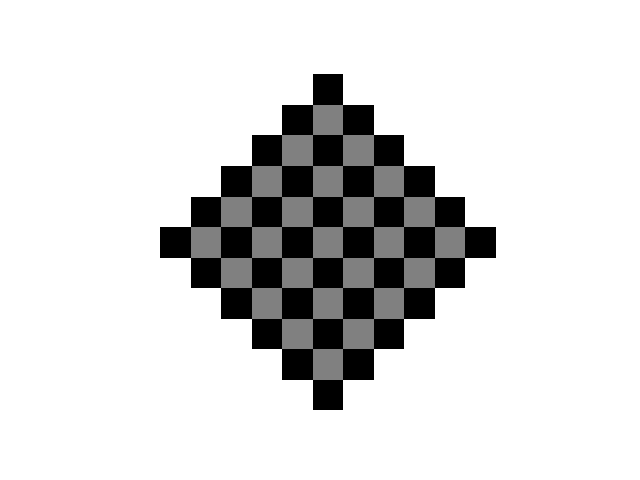
\includegraphics[width=\textwidth]{parity.png}

\end{frame}

\begin{frame}
\frametitle{Day 21: Instance}

Let's look at our instance of the problem. \vfill

Note the structure of our maze has a lot of regularity.\vfill

Also, while the full number of steps is too large to brute force,
we can solve many smaller instances.\vfill

Here is the data in Mathematica.
\end{frame}
